\documentclass[a4paper,12pt]{article}
\usepackage{graphicx}
\usepackage{cmap}
\usepackage[T2A]{fontenc}
\usepackage[utf8]{inputenc}

%%\renewcommand{\footrulewidth}{ .0em }
\usepackage[english,russian]{babel}
\usepackage{multirow} % Слияние строк в таблице
\newcommand
{\un}[1]
{\ensuremath{\text{#1}}}



\begin{document}

\begin{titlepage}
	\begin{center}
		\large 	Московский физико-технический университет \\
		Физтех-школа радиотехники и компьютерных технологий\\
		\vspace{0.2cm}
		
		\vspace{4.5cm}
		Лабораторная работа № 3.2.4 \\ \vspace{0.2cm}
		\LARGE \textbf{Свободные колебания в электрическом контуре}
	\end{center}
	\vspace{2.3cm} \large
	
	\begin{center}
		Работу выполнил: \\
		Шурыгин Антон \\
		Б01-909

		
	\end{center}
	
	\begin{center} \vspace{60mm}
		г. Долгопрудный \\
		 2020 год
	\end{center}
\end{titlepage}




\paragraph*{Цель работы:} исследование свободных колебаний в электрическом контуре.

\paragraph*{Оборудование:} генератор импульсов, электронное реле, магазин сопротивлений, магазин емкостей, индуктивность, электронный осциллограф, мост.



\section{Теоретическое введение}

\begin{figure}[h]
	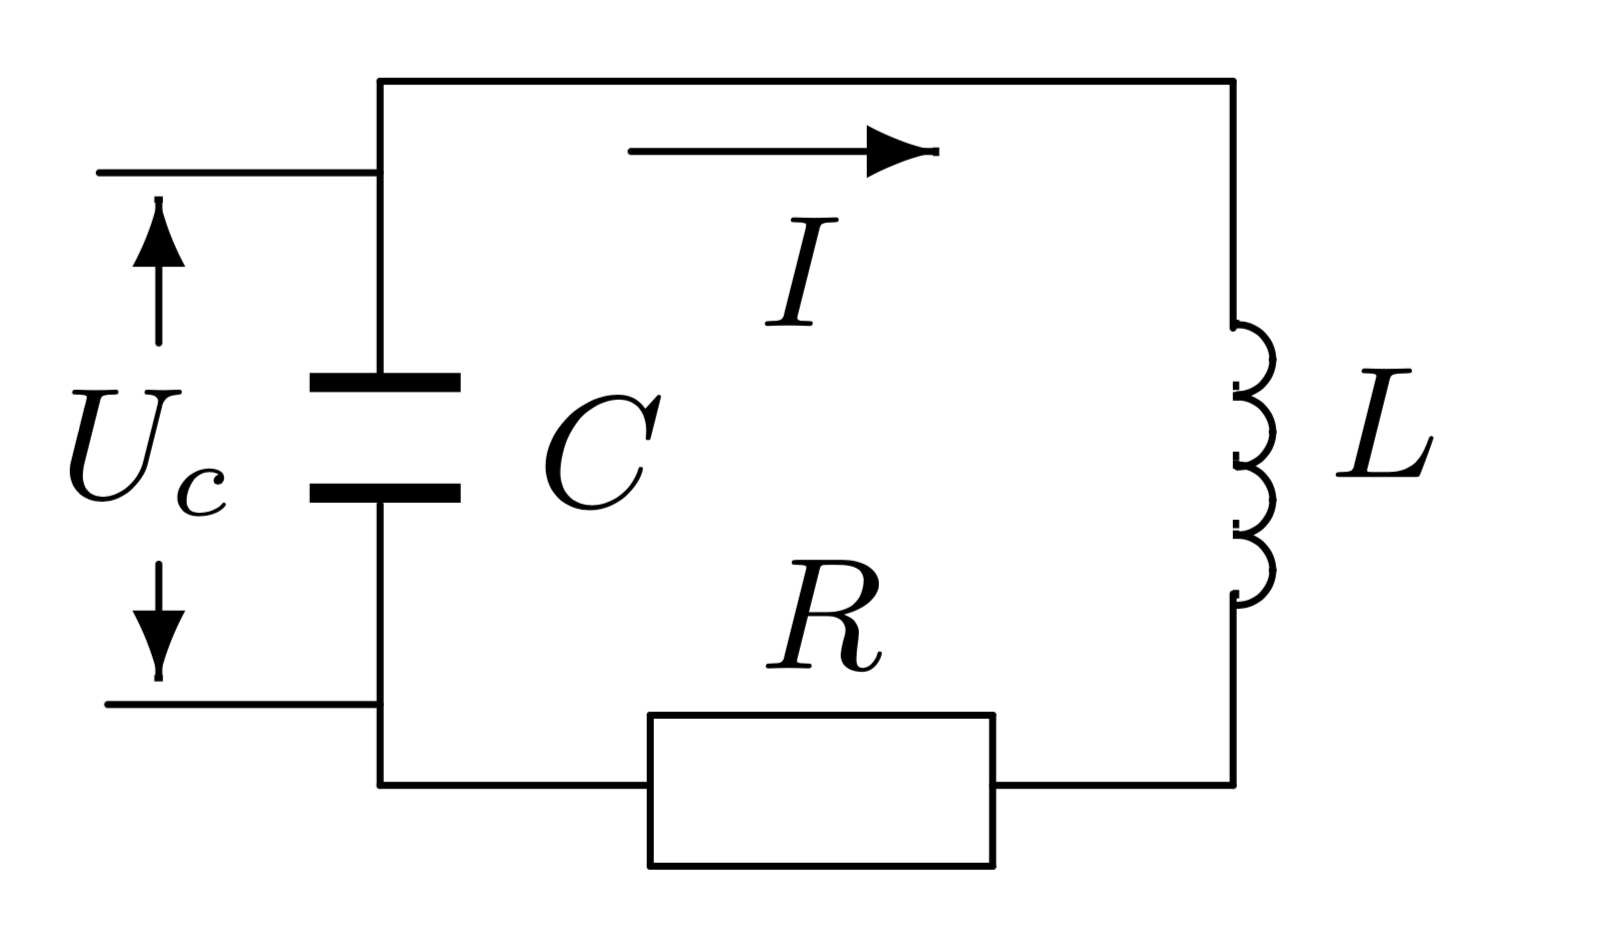
\includegraphics[width=5cm]{RLC.png}
	\caption{Колебательный контур}
	\label{RLC}
\end{figure}


Основное уравнение колебательного контура:

\begin{equation}\label{ddot I}
    \ddot{I} + 2\gamma\dot{I} + \omega_0^2I = 0
\end{equation}

Где ${\gamma = \frac{R}{2L}}$ --- коэффициент затухания, $ \omega_0^2 = \frac{1}{LC} $ --- собственная частота контура. Решением этого уравнения являются затухающие колебания:

\begin{equation}\label{}
I = A e^{-\gamma t} \cos (\omega t - \theta)
\end{equation}

Здесь $ \omega = \sqrt{\omega_0^2 - \gamma^2} $. Можно записать решение и для напряжения:

\begin{equation}\label{}
U_C = U_0 \frac{\omega_0}{\omega} e^{-\gamma t}\cos (\omega t - \theta)
\end{equation}

В контуре со слабым затуханием $ (\omega \approx \omega_0) $ верна \textbf{формула Томпсона} для периода: 

\begin{equation}\label{}
T = \frac{2\pi}{\omega_0} \approx \frac{2\pi}{\omega} = 2\pi\sqrt{LC}
\end{equation}

Режим работы контура, при котором $ \gamma = \omega_0 $, называется \textbf{критическим}. Его сопротивление равно 

\begin{equation}\label{}
R_{kr} = 2\sqrt{\frac{L}{C}}
\end{equation}

Потери затухающих колебаний принято характеризовать через \textbf{добротность} и \textbf{логарифмический декремент затухания}: 

Добротность, потери энергии:
\begin{equation}\label{Q}
Q = 2\pi \frac{W}{\Delta W} = \frac{1}{R} \sqrt{\frac{L}{C}} \quad 
\end{equation}

Лог. декремент, потери амплитуды:
\begin{equation}\label{theta}
\Theta = \frac{1}{n} \gamma T = \frac{1}{n} \ln \frac{U_k}{U_{k+n}}
\end{equation}

\section{Экспериментальная установка}

Исследуемый колебательный контур состоит из индуктивности $ L $,
ёмкости $ С $ и резистора $ R $ (рис. \ref{RLC}). Конденсатор контура заряжается
короткими одиночными импульсами, после каждого из которых в контуре
возникают свободные затухающие колебания. Подав напряжение
с конденсатора на осциллограф, можно по картине, возникающей на
экране осциллографа, определить период колебаний в контуре, исследовать
затухание колебаний и определить основные параметры колебательного
контура.

Картину колебаний можно представить не только в координатах ($ U, t $), но и в координатах ($ U, \dot{U} $), или, как говорят, на фазовой
плоскости. В этих координатах кривая незатухающих колебаний ( $ \gamma = 0 $)
имеет вид эллипса (или окружности - при одинаковых амплитудах $ U $
и $ \dot{U} $), а картина реальных колебаний изображается сворачивающейся
спиралью. 


\begin{figure}[h]
	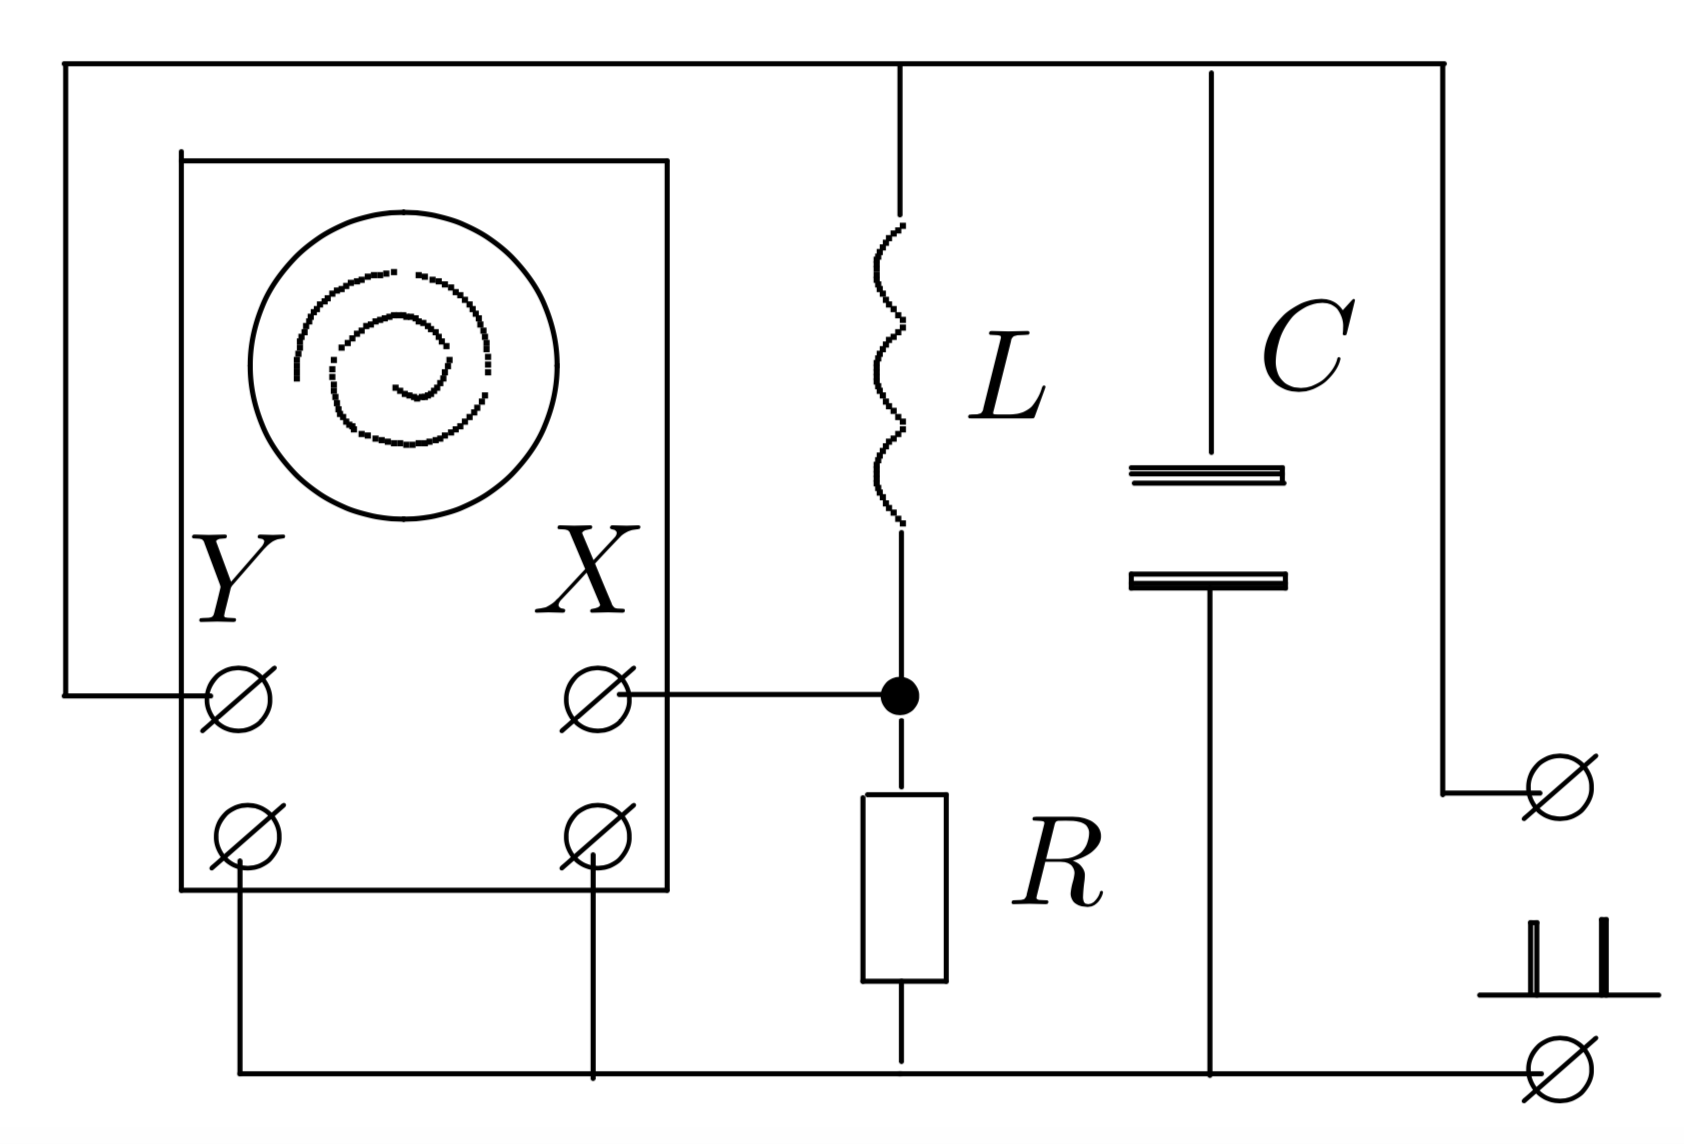
\includegraphics[width=6cm]{Fase.png}
	\caption{Фазовый режим}
	\label{Fase}
\end{figure}

Схема подключения осциллографа для изучения колебаний на фазовой плоскости представлена на рис. \ref{Fase}. На вертикальный вход осциллографа подаётся напряжение $ U_C $ с конденсатора, а на горизонтальный --- напряжение с резистора $ U_R $.

На рис. 3 приведена схема для исследования свободных колебаний в контуре типа рис. \ref{RLC}. Колебания наблюдаются на экране осциллографа.

Для периодического возбуждения колебаний в контуре используется
генератор импульсов Г5-54. С выхода генератора по коаксиальному кабелю импульсы поступают на колебательный контур через электронное
реле, смонтированное в отдельном блоке ( или на выходе генератора).
Реле содержит диодный тиристор1 $ D $ и ограничительный резистор $ R_1 $.
Импульсы заряжают конденсатор $ С $. После каждого импульса генератор
отключается от колебательного контура, и в контуре возникают
свободные затухающие колебания. Входное сопротивление осциллографа
велико ($ \backsimeq 1$ МОм), так что его влиянием иа контур можно пренебречь.

\begin{figure}[h]
	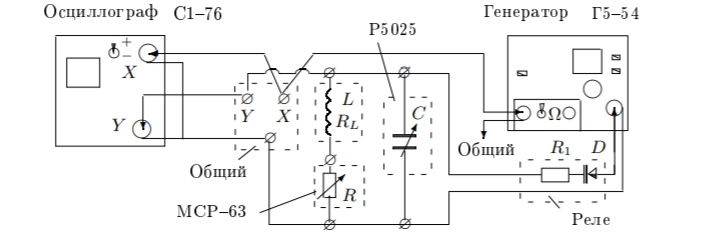
\includegraphics[width=15cm]{scheme.jpg}
	\caption{Схема экспериментальной установки}
	\label{scheme}
\end{figure}

Для получения устойчивой картины затухающих колебаний используется
режим ждущей развёртки с синхронизацией внешними импульсами,
поступающими с выхода "<синхроимпульсы"> генератора.

\section{Ход работы}

\subsection{Измерение периодов}

Проведем измерения при ${R = 0}$. Будем изменять емкость от ${0,02}$ до ${0,9}$ мкФ, проводя измерения периода по формуле:

\begin{equation}\label{}
T_{exper} = T_0 \frac{x}{nx_0}
\end{equation}

где $ T_0 = 0,01 $ c, $ x_0 $ --- длина одного импульса, $ x $ --- длина $ n $ импульсов. Погрешность $ \sigma_x = \sigma_{x_0} = 0,1, \sigma_{T_0} = 0,001  $c. Тогда 

\begin{equation}\label{}
\sigma_{T_{exper}} = T_{exper}\sqrt{ \left( \frac{ \sigma_x}{x} \right)^2 + \left( \frac{ \sigma_{x_0}}{x_0} \right)^2  +  \left( \frac{ \sigma_{T_0}}{T_0} \right)^2}
\end{equation}

А $ T_{теор} = 2\pi\sqrt{LC} $, где ${L = 200}$ мГн, $ \sigma_L = 7 $ мГн.

Тогда 

\begin{equation}\label{}
\sigma_{T_{theor}} = \frac{1}{2}\cdot{T_{theor}}} \frac{\sigma_L}{L}
\end{equation}

Результаты сведем в таблицу \ref{resT} и построим график рис. 4. 

\begin{table}[h!]
	\centering
	\caption{Результаты измерений}
	\begin{tabular}{|c|c|c|c|c|c|c|c|}
		\hline
		С, мкФ & x & x_0 & T_{exper}, мс & $\sigma_{T_{exper}}$, мс & T_{theor}, мс & $ \sigma_{T_{theor}} $, мс \\
		\hline
		0.02 & 0.6 & 5.0 & 0.35 & 0.07 & 0.4 & 0.01 \\
		0.13 & 0.9 & 5.0 & 0.88 & 0.13 & 1.01 & 0.02 \\
		0.25 & 3.5 & 5.0 & 1.20 & 0.13 & 1.4 & 0.03 \\
		0.37 & 3.0 & 5.0 & 1.50 & 0.16 & 1.71 & 0.03 \\
		0.49 & 3.3 & 5.1 & 1.67 & 0.18 & 1.97 & 0.03 \\
		0.61 & 4.0 & 5.1 & 1.90 & 0.20 & 2.19 & 0.04 \\
		0.75 & 4.3 & 5.1 & 2.10 & 0.22 & 2.43 & 0.04 \\
		0.90 & 4.5 & 5.1 & 2.30 & 0.24 & 2.67 & 0.05 \\
		\hline
	\end{tabular}% 
\label{resT}% 
\end{table}% 

Воспользуемся формулами LS для коэффициентов оптимальной прямой $y = ax + b$:


\begin{equation}\label{}
b = \frac{\left\langle{xy}\right\rangle - \left\langle{x}\right\rangle \left\langle{y}\right\rangle}{\left\langle{x^2}\right\rangle - \left\langle{x}\right\rangle^2}
\end{equation}

\begin{equation}\label{}
a = \left\langle{y}\right\rangle - b\left\langle{x}\right\rangle
\end{equation}

\begin{equation}\label{}
\sigma_{b} = \frac{1}{\sqrt{n}}\sqrt{\frac{\left\langle{y^2}\right\rangle - \left\langle{x}\right\rangle^2}{\left\langle{x^2}\right\rangle - \left\langle{x}\right\rangle^2} - b^2}
\end{equation}

\begin{equation}\label{}
\sigma_{a} = \sigma_{b}\sqrt{\left\langle{x^2}\right\rangle - \left\langle{x}\right\rangle^2}
\end{equation}

\begin{table}[h!]%{l}{0.5\linewidth}
	\centering
	\caption{Расчет апроксимированной прямой $ y = ax +b $}
	\begin{tabular}{c|cc}
		\text{} & \text{Estimate} & \text{Error} \\
		\hline
		b & -0.005 & 0.00025  \\
		a & 1.162 & 0.005     \\
	\end{tabular}
\end{table} 

\begin{figure}[h!]
	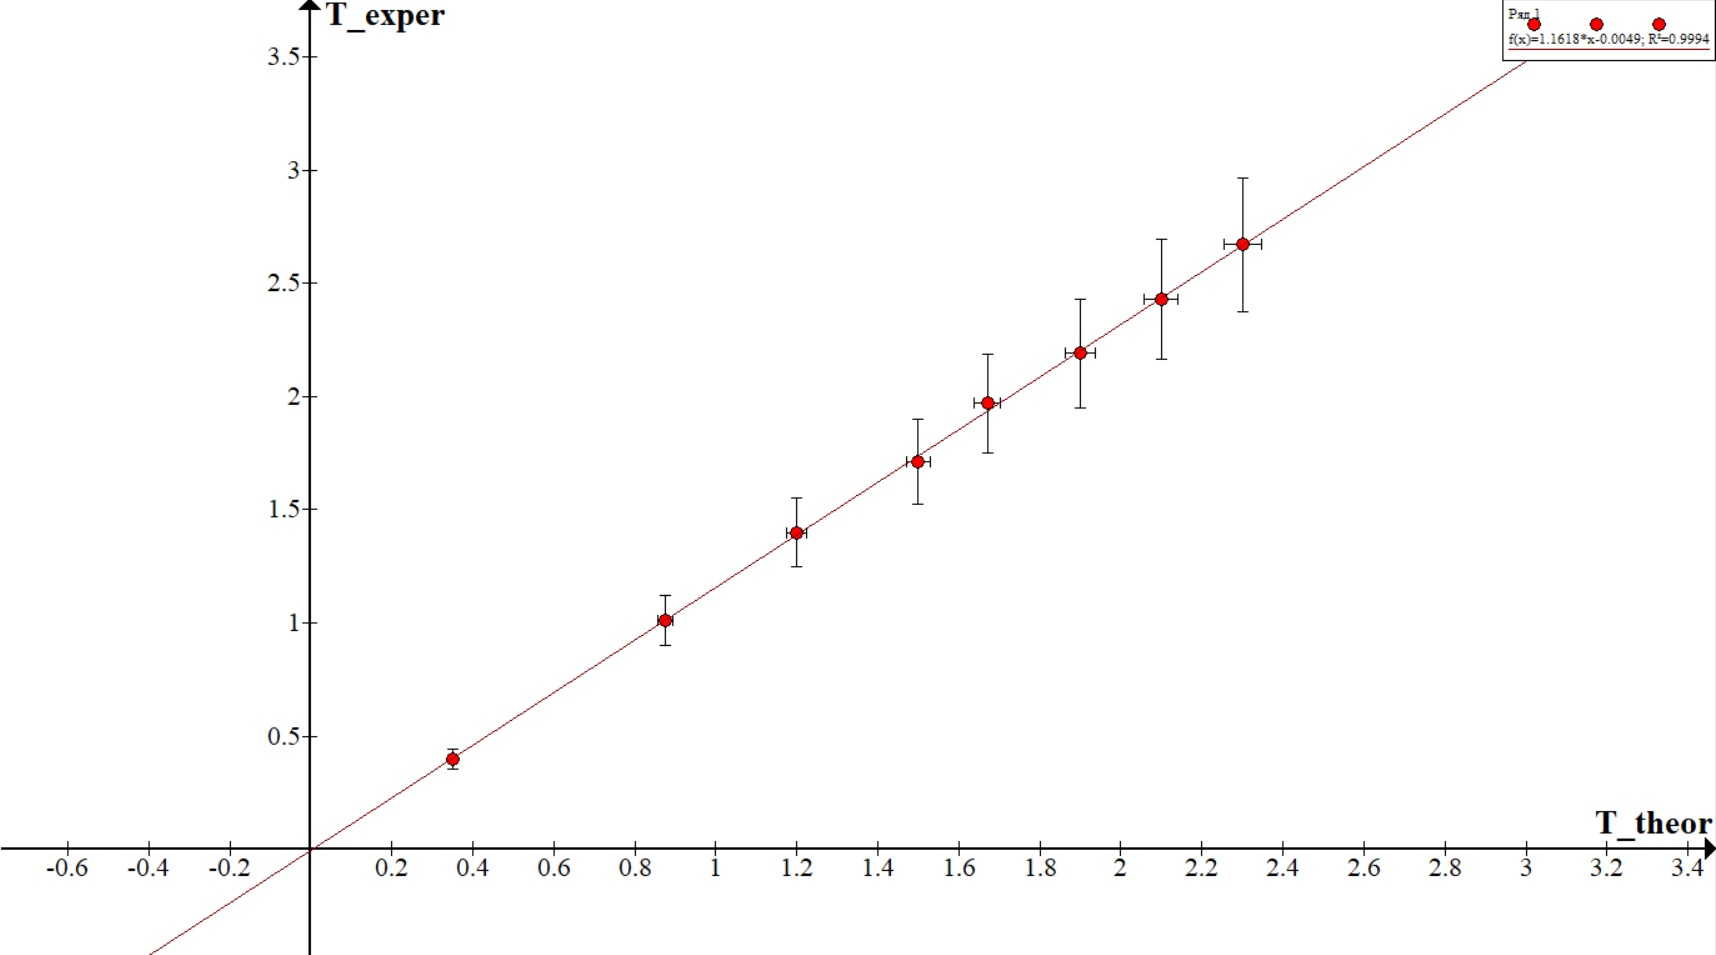
\includegraphics[scale=0.44]{lab324.jpg}
	\
	\caption{Зависимость $ T_{theor}$ от $ T_{exper} $}
\end{figure}

\subsection{Критическое сопротивление и декремент затухания}

Теперь, считая $ L = 200 $ мГн, вычислим  частоту емкость, считая $ \nu_0 = \frac{1}{LC} = 5 $ кГц $ \te C = 5  $ нФ. Тогда 
 
 \begin{equation}\label{}
 R_{krit} \approx 12,6 \space kOm
 \end{equation}

Установим эту $ С $ на магазине емкостей, будем наблюдать картину затухающих колебаний, изменяя $ R $ от $ 0,1 R_{кр}$ до $ R_{кр} $. Сопротивление магазина, при котором колебания переходят в апериодический, примерно равен критическому. 

Физический смысл логорифмического декремента затухания: это величина, обратная числу периодов $ n $, за которое амплитуда колебаний падает в $ e $ раз.


\subsection{Добротность}
Добротность контура показывает, во сколько раз запасенная в контуре энергия превосходит среднюю потерю энергии  за время, в течение которого фаза колебаний изменится на один радиан.


\section{Вывод}

В этой работе мы изучили свободные колебания в электрическом контуре: сначала измеряли периоды при $ \gamma \approx 0 $.
Затем, найдя по формуле {(15)} критическое сопротивление, постепенно увеличивали сопротивление в магазине до тех пор, пока не достигли $R_{krit}$.

Увидели картину апериодических колебаний (т.е. ${\gamma \gg \omega_{0}}$).
\newline
Так же увидели в координатах $j(u)$ cпираль.


\end{document}